\section{Introduction}
\label{sec:intro}
Text‑to‑video (T2V) generation has advanced rapidly, with large‑scale
models now producing visually impressive clips from short textual
prompts \cite{zheng2024open, yang2024cogvideox, chen2024videocrafter2, wang2025wan}.
A critical shortcoming remains unresolved: state‑of‑the‑art
T2V systems frequently violate basic physical commonsense even when the
visual quality is high.
Objects may teleport, ignore gravity, or pass
through each other, violating real‑world physics.
Recent evaluations \cite{meng2024towards, bansal2024videophy, Bansal2025} report major physical inconsistencies, showing that top
public models still struggle with scenarios requiring mass and momentum conservation laws.
This gap between visual realism and physical plausibility severely limits their deployment in domains that demand fidelity to real‑world dynamics (e.g.\ robotics and simulation).

One root cause is a mismatch between how T2V models are trained and how they are used. During training, models ingest detailed, carefully crafted captions paired with videos. However, real prompts are often brief or underspecified at inference, yielding suboptimal outputs \cite{xue2024phyt2v, cheng2025vpo}.
For instance, a user might write "\textit{A wine is poured from a bottle in to a glass}" and obtain a video where wine flows from the bottle but the liquid level in the glass remains nearly unchanged (Figure~\ref{fig:demo}, top row). While this prompt achieves high semantic adherence (Semantic score:5), it suffers from poor physical commonsense (Phyiscal score:3). Crucially, \emph{manually rewriting} the prompt to include explicit physical details such as "\textit{The level in the glass rises steadily}" successfully produces physically plausible videos where the liquid accumulates visibly (Figure~\ref{fig:demo}, second row), achieving perfect scores (Semantic score:5, Phyiscal score:3). This demonstrates that current T2V generators \emph{possess the capability} to synthesize physically realistic content when provided with physics-aware prompts; the bottleneck lies in the prompt itself. However, manual prompt engineering requires domain expertise, is time-consuming, and does not scale to diverse scenarios.

Existing automated approaches partially address this gap but face key limitations.
Promptist \cite{hao2023promptist} automatically enhances user
inputs for text‑to‑image models via supervised fine‑tuning followed by reinforcement learning
(RL) on aesthetic rewards, but does not target physical plausibility.
Early text‑to‑video work employs large language models (LLMs) such as GPT‑4o to enhance prompts through in‑context learning; while these methods can improve physics adherence (e.g., GPT‑4o achieves PC:5 in ~\cref{fig:demo}), they may reduce semantic fidelity (SA:4) and lack systematic optimization for video‑level physical commonsense.
VPO~\cite{cheng2025vpo} refines prompts with preference‑based RL to ensure they are harmless and accurate, but, like Promptist, does not explicitly address physical plausibility.
Very recently, PhyT2V introduced an LLM-guided, iterative self-refinement loop that enables chain-of-thought and "step-back" reasoning in T2V prompting, improving adherence to real-world physics and outperforming prior prompt enhancers on out-of-distribution scenarios~\cite{xue2024phyt2v}.
While PhyT2V demonstrates the value of iterative LLM feedback, it requires multiple prompting rounds and a complex step-back mechanism, limiting its efficiency.

\begin{figure*}[t]
    \centering
    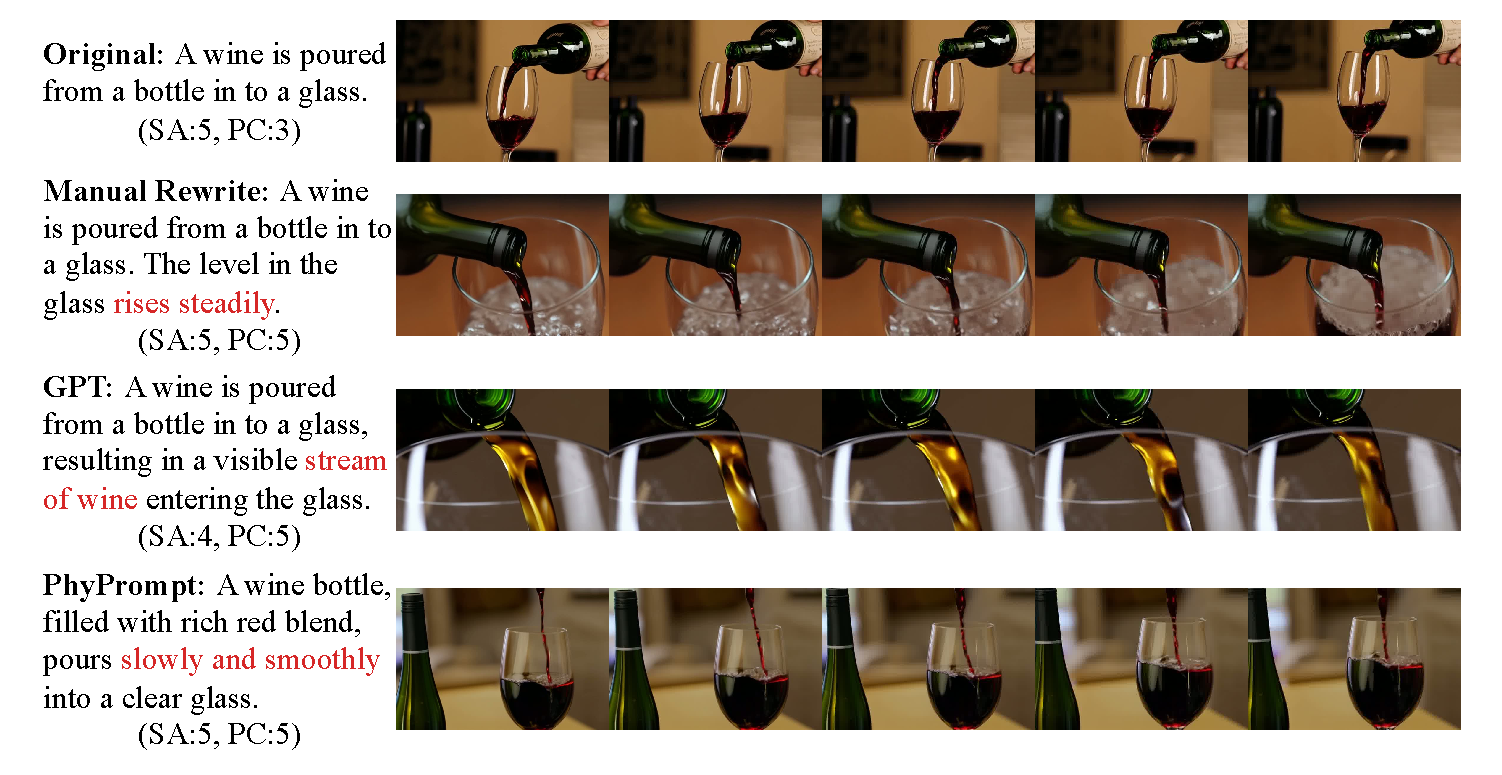
\includegraphics[width=\textwidth]{figures/prompt_demo.pdf}
    \caption{\textbf{Video Generated by CogVideoX-5B Using Different Prompts.} We compare the original prompt \textit{A wine is poured from a bottle in to a glass} with three enhanced versions: manual rewrite, GPT-4o, and PhyPrompt.  Semantic Adherence (SA) and Physical Commonsense (PC) scores are shown for each. The original prompt fails to depict rising liquid levels (PC:3). Manual rewriting with "rises steadily" achieves perfect scores (SA:5, PC:5). GPT-4o emphasizes the "visible stream of wine" but slightly reduces semantic alignment (SA:4, PC:5). PhyPrompt automatically generates "slowly and smoothly," matching manual rewrite quality (SA:5, PC:5) without human intervention.}
    \label{fig:demo}
\end{figure*}

To address these limitations, we introduce \textbf{PhyPrompt}, a novel framework that leverages a Large Language Model (LLM) trained with reinforcement learning (RL) to \emph{automatically} transform user prompts into descriptions that elicit physically realistic video outputs, matching the quality of manual physics-aware prompt engineering without requiring human expertise.
Our approach is characterized by a two-stage training pipeline.
First, the LLM undergoes Supervised Fine-Tuning (SFT) on a high-quality, Chain-of-Thought (CoT) dataset curated by us, based on PhyGenBench \cite{meng2024towards}.
This dataset is specifically designed to imbue the LLM with the ability to reason about physical phenomena and translate these considerations into descriptive text suitable for video generation.
In the second stage, the SFT-trained LLM's prompt generation policy is further refined using Group Relative Policy Optimization (GRPO)~\cite{guo2025deepseek}, an RL algorithm that efficiently explores the prompt space by sampling multiple candidates per query without requiring a separate value network.

A key innovation in PhyPrompt is its dynamic reward mechanism inspired by curriculum training \cite{bengio2009curriculum}.
The GRPO training is guided by a composite reward signal that adaptively balances the physical commonsense of the generated video and its semantic alignment with the user's intent.
In our design, the reward prioritizes semantic alignment in the early stages of training, gradually shifting the emphasis towards physical commonsense as the LLM's policy matures.
This curriculum-like approach ensures that the LLM first learns to preserve the user's intent before focusing on the more nuanced task of enhancing physical realism.
Our architecture leaves the video generator frozen and trains only a lightweight, model‑agnostic rewriter that converts user prompts into physics‑aware descriptions.
This avoids costly generator fine‑tuning and allows one rewriter to serve multiple back‑ends.

We validate our approach on four cutting‑edge generators: Lavie~\cite{wang2023lavie}, VideoCrafter2~\cite{chen2024videocrafter2}, CogVideoX-2B and CogVideoX-5B~\cite{wang2024cogvideodex}.
For each, we insert the trained LLM between the user and the generator.
Experiments on the test dataset from VideoPhy2 dataset show that rewritten prompts reduce physics violations while maintaining visual quality and semantic fidelity.
As demonstrated in~\cref{fig:demo}, PhyPrompt automatically generates prompts that achieve the same level of physical plausibility (PC:5) and semantic adherence (SA:5) as manually engineered physics-aware prompts, eliminating the need for human expertise in prompt design.
The main contributions of this work are as follows:
\begin{itemize}
    \item We demonstrate that current T2V generators can produce physically plausible videos when provided with physics-aware prompts, and propose PhyPrompt, a novel two-stage trained LLM system.
    \item We introduce a dynamic, time-dependent reward mechanism for RL-based prompt optimization that progressively shifts focus from semantic alignment to physical commonsense, facilitating a balanced and effective learning curriculum.
      \item Empirical validation showing zero-shot transfer across multiple T2V models, with joint semantic-adherence and physical-commonsense gains of up to 16.8\%, achieving quality comparable to manual physics-aware prompt engineering.
\end{itemize}
